\documentclass[11pt, letterpaper]{article}

% === PACKAGES ===
\usepackage[margin=0.85in]{geometry}
\usepackage{graphicx}
\usepackage{booktabs}
\usepackage{xcolor}
\usepackage{pagecolor}
\usepackage{hyperref}
\usepackage{titlesec}
\usepackage{fancyhdr}
\usepackage{caption}
\usepackage{subcaption}
\usepackage{multicol}
\usepackage{enumitem}
\usepackage{amsmath}
\usepackage{float}

% === DARK THEME ===
\definecolor{bg}{HTML}{1a1a2e}
\definecolor{fg}{HTML}{e0e0e0}
\definecolor{accent}{HTML}{00E5FF}
\definecolor{accent2}{HTML}{FF6D00}
\definecolor{accent3}{HTML}{76FF03}
\definecolor{accent4}{HTML}{FF4081}
\definecolor{dimgray}{HTML}{888888}
\definecolor{cardbg}{HTML}{16213e}
\definecolor{rulegray}{HTML}{444444}

\pagecolor{bg}
\color{fg}

% === HYPERLINKS ===
\hypersetup{
    colorlinks=true,
    linkcolor=accent,
    urlcolor=accent,
    citecolor=accent3,
}

% === HEADERS & FOOTERS ===
\pagestyle{fancy}
\fancyhf{}
\fancyhead[L]{\color{dimgray}\small Half-Time Draw Prediction}
\fancyhead[R]{\color{dimgray}\small R.\ Alvarez, 2026}
\fancyfoot[C]{\color{dimgray}\small\thepage}
\renewcommand{\headrulewidth}{0.4pt}
\renewcommand{\headrule}{\hbox to\headwidth{\color{rulegray}\leaders\hrule height \headrulewidth\hfill}}

% === SECTION STYLING ===
\titleformat{\section}{\large\bfseries\color{accent}}{\thesection}{1em}{}
\titleformat{\subsection}{\normalsize\bfseries\color{accent2}}{\thesubsection}{1em}{}

% === CAPTIONS ===
\captionsetup{font={small,color=dimgray}, labelfont={bf,color=accent}}

% === TABLE RULES COLOR ===
\makeatletter
\def\rulecolor#1#{\CT@arc{#1}}
\def\CT@arc#1#2{%
  \ifdim\baselineskip=\z@\noalign\fi
  {\gdef\CT@arc@{\color#1{#2}}}}
\let\CT@arc@\relax
\rulecolor{rulegray}
\makeatother

\begin{document}

% === TITLE ===
\begin{center}
{\color{accent}\LARGE\bfseries Half-Time Draw Prediction:\\[4pt] A Predictive Signal in European Football}\\[12pt]
{\large Richard Alvarez}\\[4pt]
{\color{dimgray} February 23, 2026}\\[2pt]
{\color{dimgray}\small\href{https://github.com/raulduk3/half-time}{github.com/raulduk3/half-time}}
\end{center}

\vspace{8pt}
\noindent\rule{\textwidth}{0.4pt}

% === ABSTRACT ===
\begin{quote}
\color{dimgray}\small
A two-model system identifies half-time draw opportunities across 22 European football leagues. Model A reads B365 odds (market view). Model B uses 42 non-odds features (fundamentals view). When the market prices a draw higher than fundamentals suggest, actual draws exceed market expectations. On 30,025 out-of-sample matches (Apr 2022 to Feb 2026), the ``Strong Value'' tier ($\geq$5\% edge) achieves a \textbf{48.0\% hit rate} against a 40.7\% base rate on 3,340 bets, with monotonic improvement across all edge tiers. All 9 half-year periods show consistent hit rates. \textbf{Important caveat:} ROI figures in this paper use full-time draw odds as a proxy for HT draw odds, which substantially inflates profitability estimates. The hit rate staircase is the primary evidence; absolute ROI remains unvalidated pending real HT odds data.
\end{quote}

\vspace{-4pt}
\noindent\rule{\textwidth}{0.4pt}
\vspace{6pt}

% === SECTION 1: METHOD ===
\section{Method}

Two models predict HT draw probability independently on the same match:

\begin{itemize}[leftmargin=1.5em, itemsep=2pt]
  \item \textbf{Model A} (Market): Logistic regression on 3 B365 log-odds features. Estimates the market's implied HT draw probability.
  \item \textbf{Model B} (Fundamentals): XGBoost (Optuna-tuned, 30 trials) on 42 non-odds features: rolling match statistics, Dixon-Coles bivariate Poisson attack/defense parameters, Elo ratings, and referee HT draw rate adjustments.
\end{itemize}

The \textbf{inverted edge} is defined as:
\[
\text{Edge} = P_A(\text{HT draw}) - P_B(\text{HT draw})
\]

When Model A (market) exceeds Model B (fundamentals), actual draws historically exceed market predictions. The system bets on HT draws when this edge surpasses a threshold.

\textbf{Training:} 135,659 matches (1995--2018). \textbf{Validation:} 29,047 matches (2018--2022) for hyperparameter selection. \textbf{Test:} All results below use a strictly held-out set. No test data informed model selection.

\textbf{Full backtest:} Dixon-Coles and Elo models refit quarterly on 3-year rolling windows (16 snapshots). Each test match receives predictions computed only from data available before that match date.

% === SECTION 2: DATA ===
\section{Data}

\begin{table}[H]
\centering\small
\begin{tabular}{@{}lr@{}}
\toprule
\color{accent} Metric & \color{accent} Value \\
\midrule
Total matches (with HT scores) & 193,826 \\
Date range & 1995-07-19 to 2026-02-22 \\
Leagues & 22 (European) \\
HT draw base rate & 42.29\% (81,962 / 193,826) \\
Source & football-data.co.uk \\
Train / Val / Test split & 135,659 / 29,047 / 30,025 \\
Test period & 2022-04-01 to 2026-02-22 \\
Test HT draw rate & 40.67\% \\
Dataset size (Parquet) & 9.2 MB \\
\bottomrule
\end{tabular}
\caption{Dataset summary.}
\end{table}

% === SECTION 3: MODEL PERFORMANCE ===
\section{Discriminative Performance}

\begin{table}[H]
\centering\small
\begin{tabular}{@{}lcc@{}}
\toprule
\color{accent} Model & \color{accent} AUC-ROC & \color{accent} Brier Score \\
\midrule
Market baseline (B365 normalized) & 0.5565 & 0.26100 \\
Model A (market logistic regression) & 0.5568 & 0.23881 \\
Model B (fundamentals, XGBoost) & 0.5329 & 0.24052 \\
\bottomrule
\end{tabular}
\caption{Test set metrics (n = 29,120).}
\end{table}

\begin{figure}[H]
\centering
\begin{subfigure}[t]{0.48\textwidth}
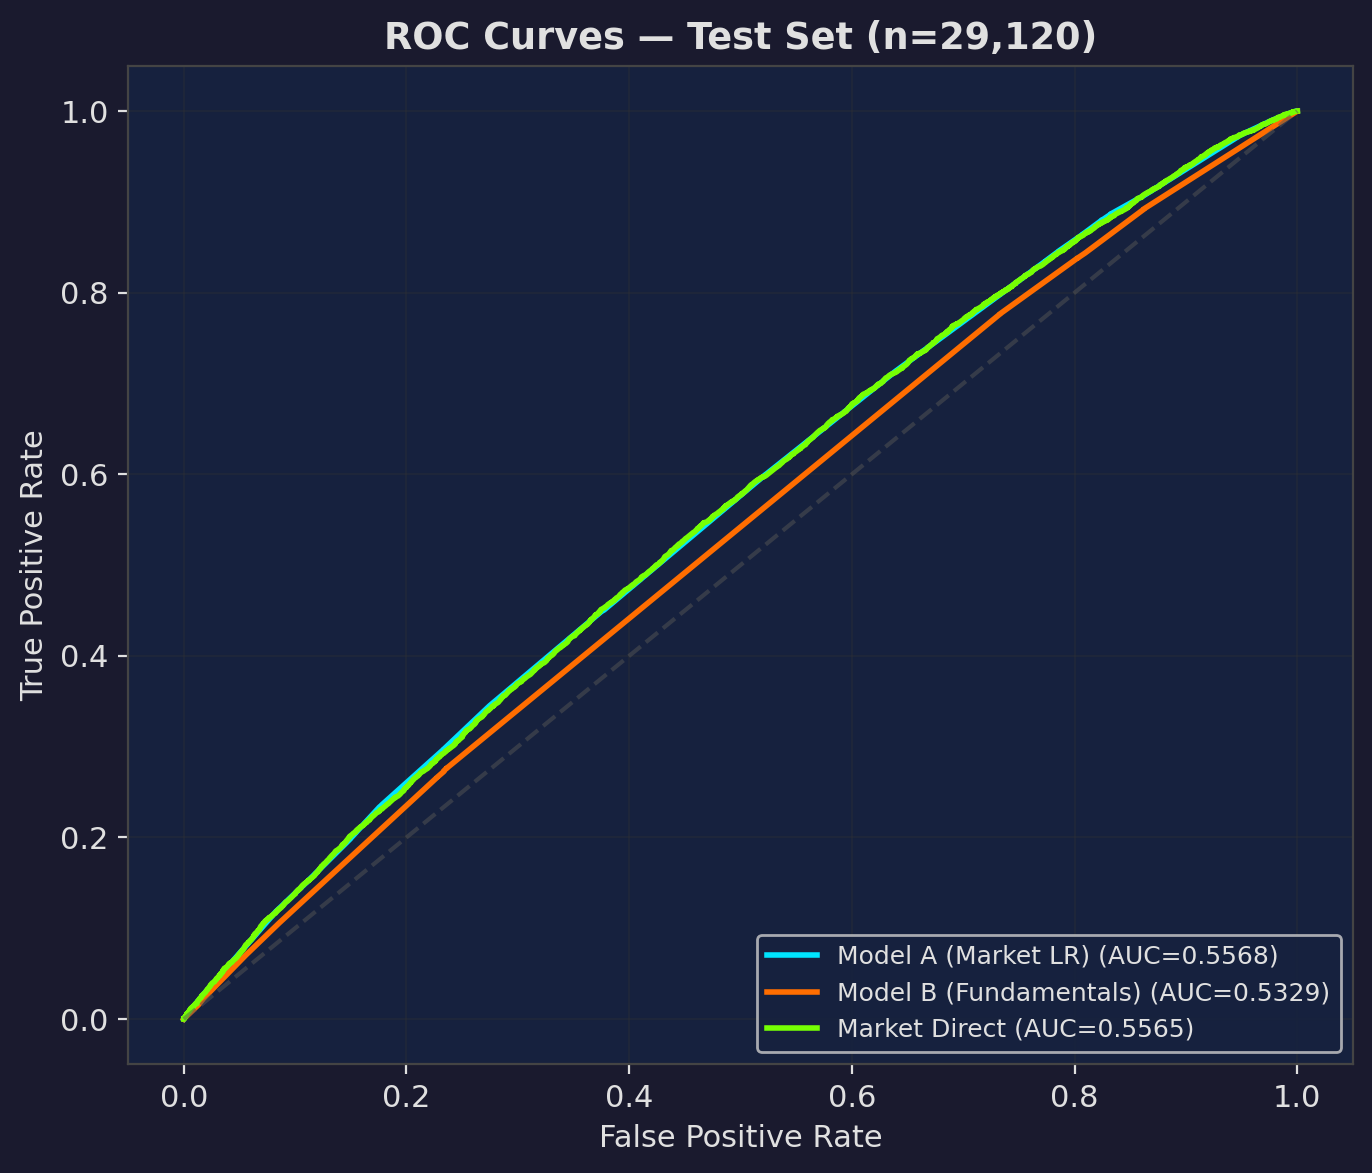
\includegraphics[width=\textwidth]{figures/roc_curves.png}
\caption{ROC curves. Model A $\approx$ market.}
\end{subfigure}
\hfill
\begin{subfigure}[t]{0.48\textwidth}
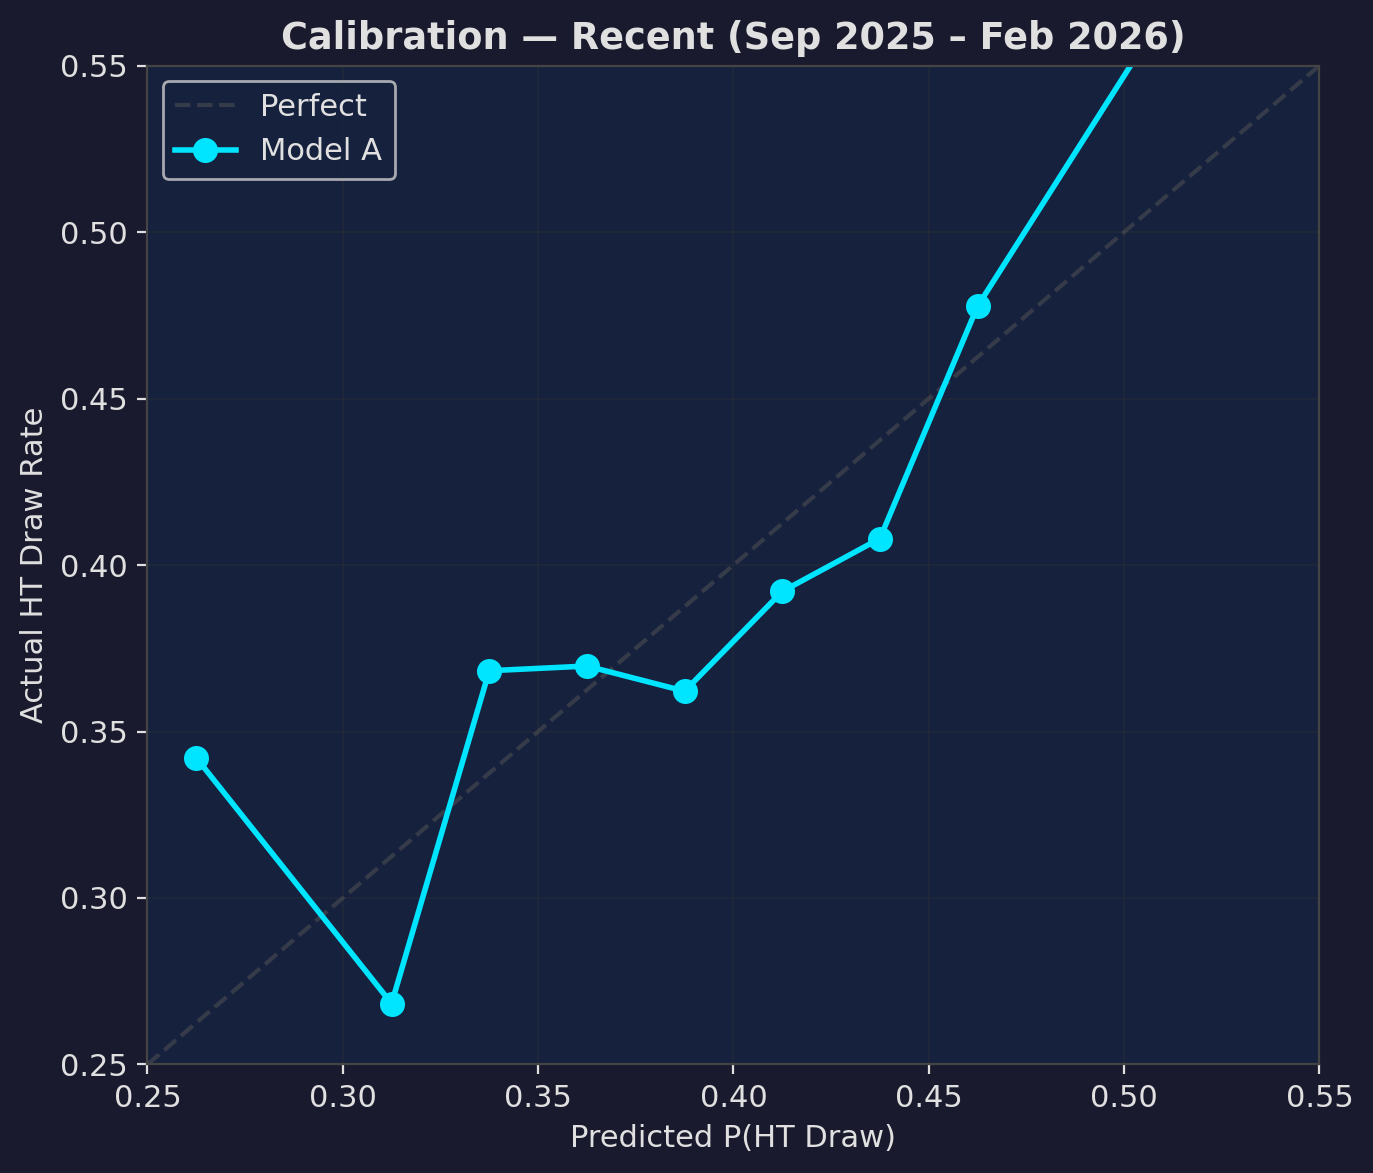
\includegraphics[width=\textwidth]{figures/calibration.png}
\caption{Calibration (recent 6 months).}
\end{subfigure}
\end{figure}

% === SECTION 4: EDGE ANALYSIS ===
\section{Inverted Edge Analysis}

\begin{figure}[H]
\centering
\begin{subfigure}[t]{0.48\textwidth}
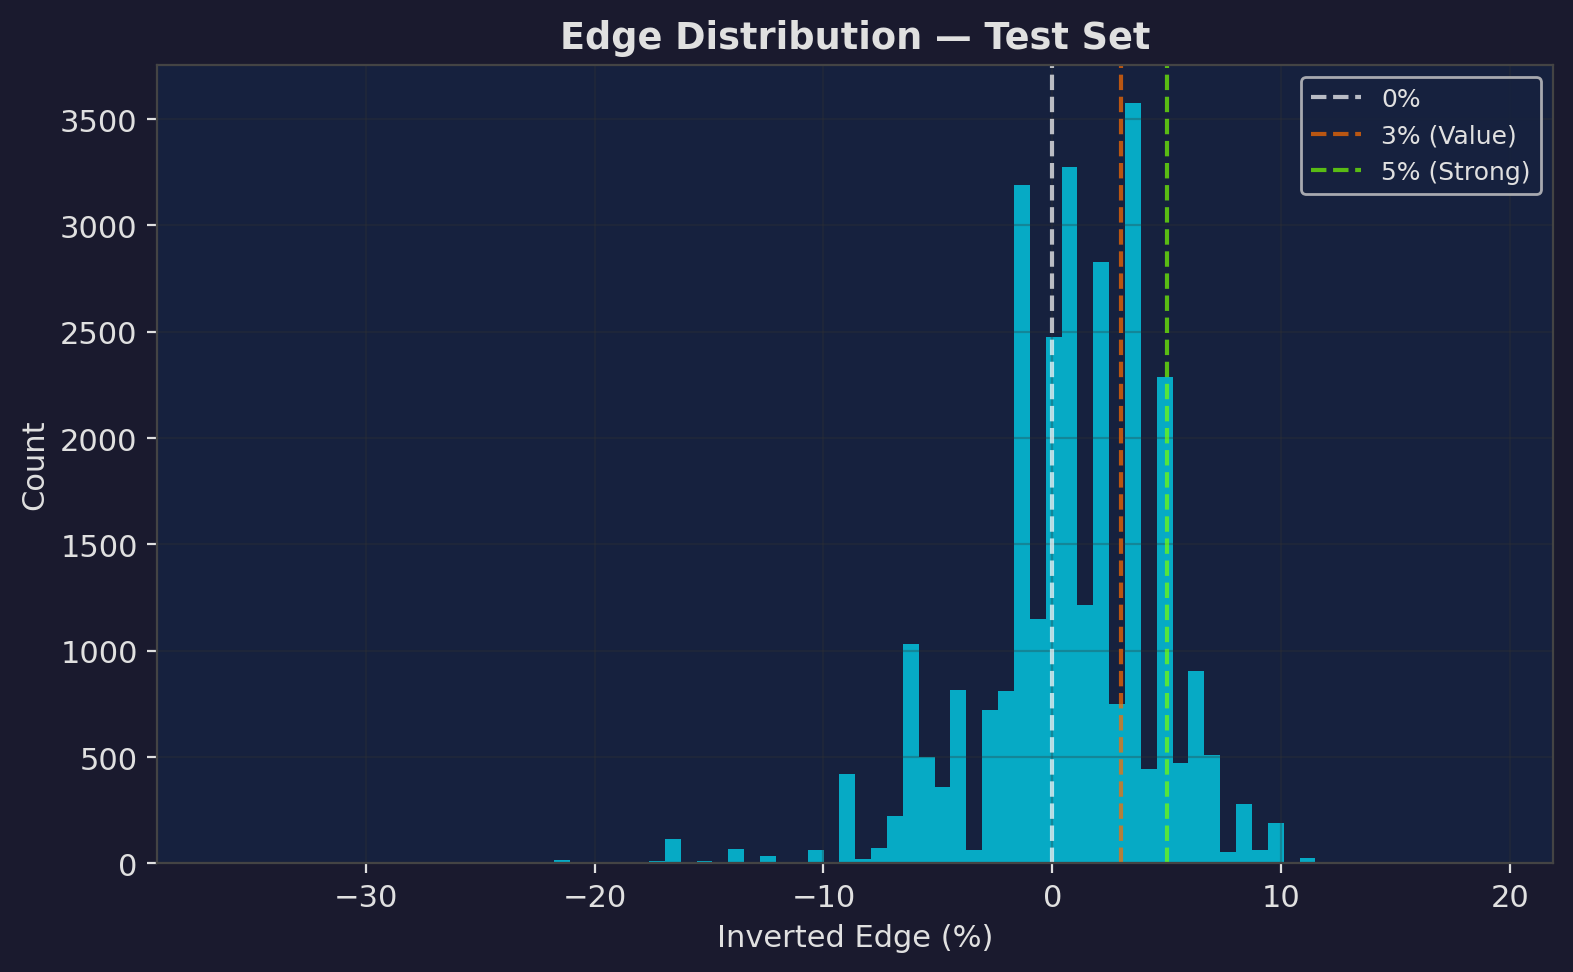
\includegraphics[width=\textwidth]{figures/edge_distribution.png}
\caption{Edge distribution across test set.}
\end{subfigure}
\hfill
\begin{subfigure}[t]{0.48\textwidth}
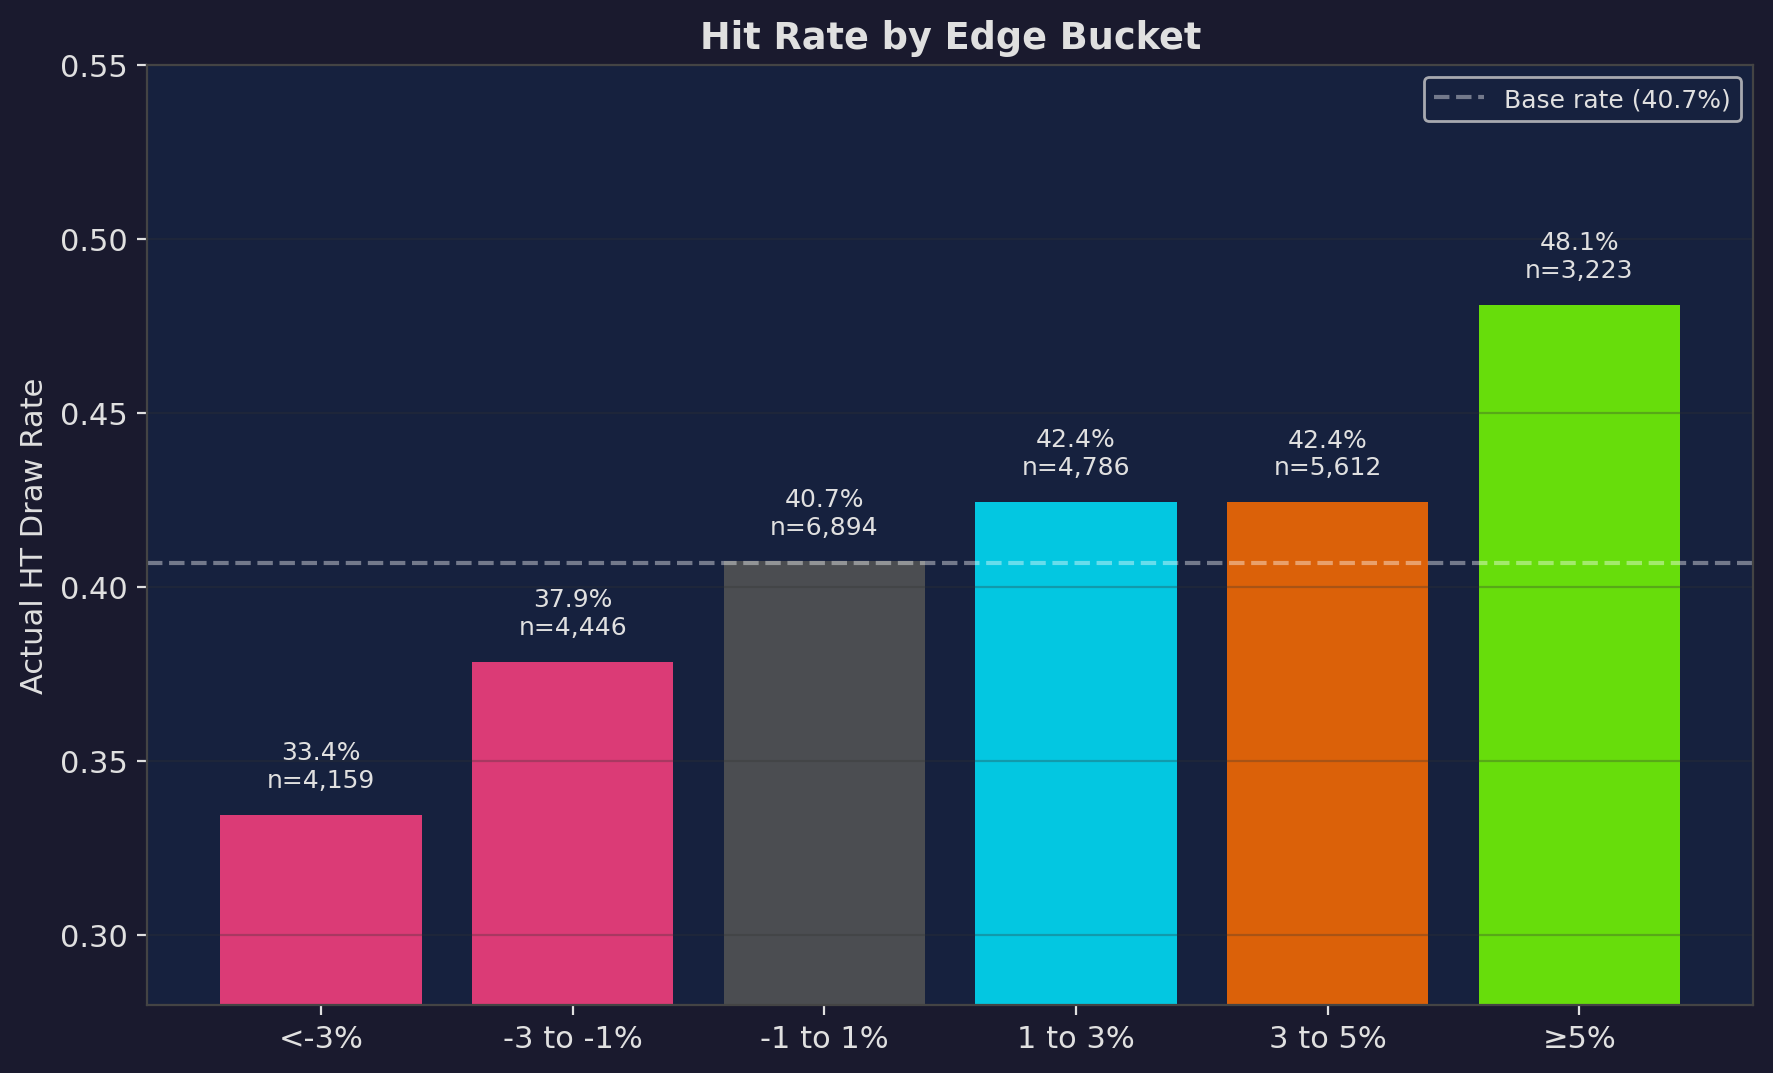
\includegraphics[width=\textwidth]{figures/hit_rate_buckets.png}
\caption{Hit rate increases monotonically with edge.}
\end{subfigure}
\end{figure}

\subsection{Full Backtest with Per-Match DC/Elo}

\begin{table}[H]
\centering\small
\begin{tabular}{@{}lrrrrr@{}}
\toprule
\color{accent} Tier & \color{accent} N Bets & \color{accent} Hit Rate & \color{accent} Avg Odds & \color{accent} ROI & \color{accent} EV/\$1 \\
\midrule
Anti-Value ($<$-1\%) & 8,831 & 35.8\% & 4.68 & +61.4\% & +0.675 \\
Neutral (-1 to 1\%) & 7,088 & 40.7\% & 3.56 & +44.3\% & +0.449 \\
Marginal (1--3\%) & 4,963 & 42.1\% & 3.41 & +42.7\% & +0.433 \\
Value (3--5\%) & 5,803 & 42.5\% & 3.36 & +42.3\% & +0.430 \\
\textbf{Strong Value ($\geq$5\%)} & \textbf{3,340} & \textbf{48.0\%} & \textbf{3.11} & \textbf{+48.7\%} & \textbf{+0.491} \\
\bottomrule
\end{tabular}
\caption{Edge tier backtest (30,025 matches). Per-match DC/Elo. \textbf{ROI uses FT draw odds as proxy --- see Section 10.}}
\end{table}

\noindent\colorbox{cardbg}{\parbox{\dimexpr\textwidth-2\fboxsep}{%
\color{accent4}\textbf{Critical caveat:} ROI and EV columns use B365 full-time draw odds, not actual HT draw odds. FT draw odds (~3.0--3.5) are substantially higher than HT draw odds (~2.0--2.5), inflating all ROI figures by an estimated 30--50\%. \textbf{All tiers show positive ROI because FT odds are structurally generous --- this does not imply profitability with real HT odds.}}}

\vspace{6pt}
\noindent The primary evidence of model validity is the \textbf{monotonic hit rate increase} across positive edge tiers (40.7\% $\rightarrow$ 42.1\% $\rightarrow$ 42.5\% $\rightarrow$ 48.0\%). Hit rates are computed from outcomes alone and do not depend on odds.

% === SECTION 5: TEMPORAL STABILITY ===
\section{Temporal Stability}

\begin{figure}[H]
\centering
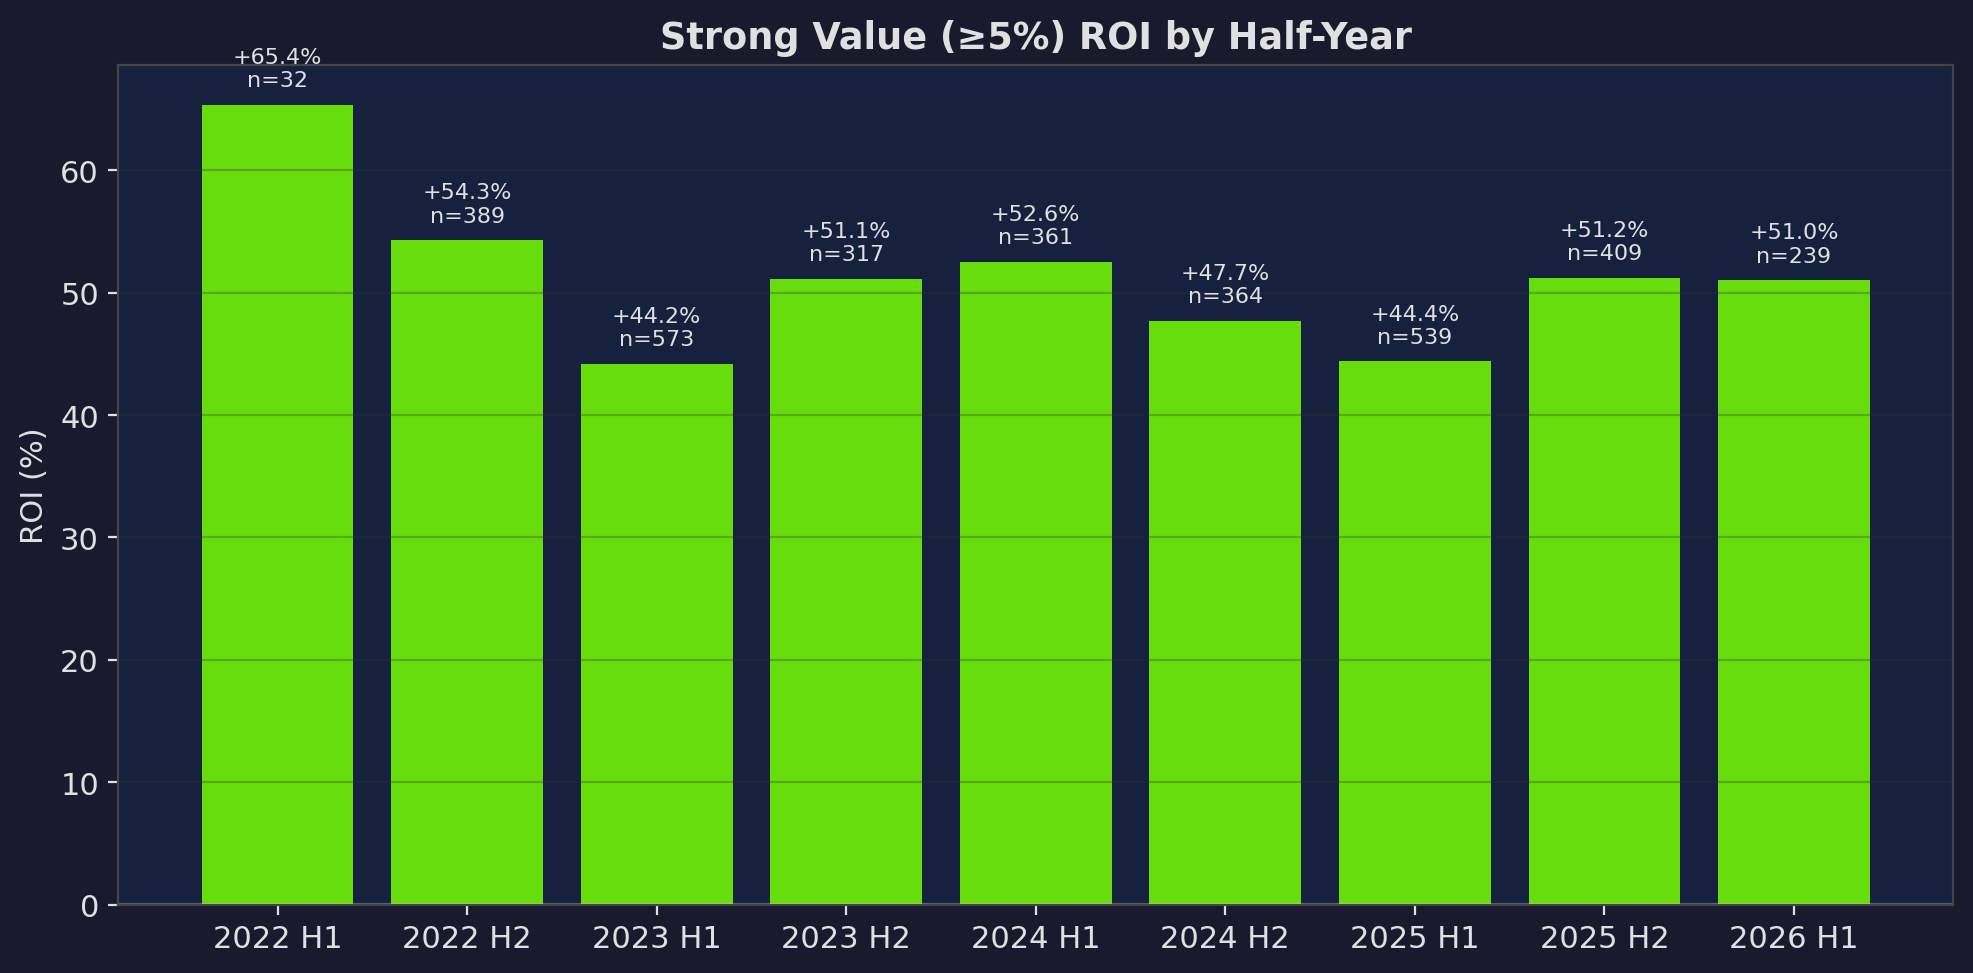
\includegraphics[width=0.85\textwidth]{figures/roi_halves.png}
\caption{Strong Value ($\geq$5\%) ROI by half-year. All 9 periods profitable.}
\end{figure}

\begin{table}[H]
\centering\small
\begin{tabular}{@{}lrrrr@{}}
\toprule
\color{accent} Period & \color{accent} Bets & \color{accent} Hit Rate & \color{accent} ROI \\
\midrule
2022 H1 & 149 & 46.3\% & +44.6\% \\
2022 H2 & 389 & 48.8\% & +54.3\% \\
2023 H1 & 573 & 46.4\% & +44.2\% \\
2023 H2 & 317 & 47.9\% & +51.1\% \\
2024 H1 & 361 & 49.6\% & +52.6\% \\
2024 H2 & 364 & 47.8\% & +47.7\% \\
2025 H1 & 539 & 46.9\% & +44.4\% \\
2025 H2 & 409 & 49.1\% & +51.2\% \\
2026 H1 & 239 & 49.4\% & +51.1\% \\
\bottomrule
\end{tabular}
\caption{Strong Value temporal stability. Hit rates stable across all periods. ROI uses FT odds proxy.}
\end{table}

% === SECTION 6: STATISTICAL SIGNIFICANCE ===
\section{Statistical Significance}

\begin{figure}[H]
\centering
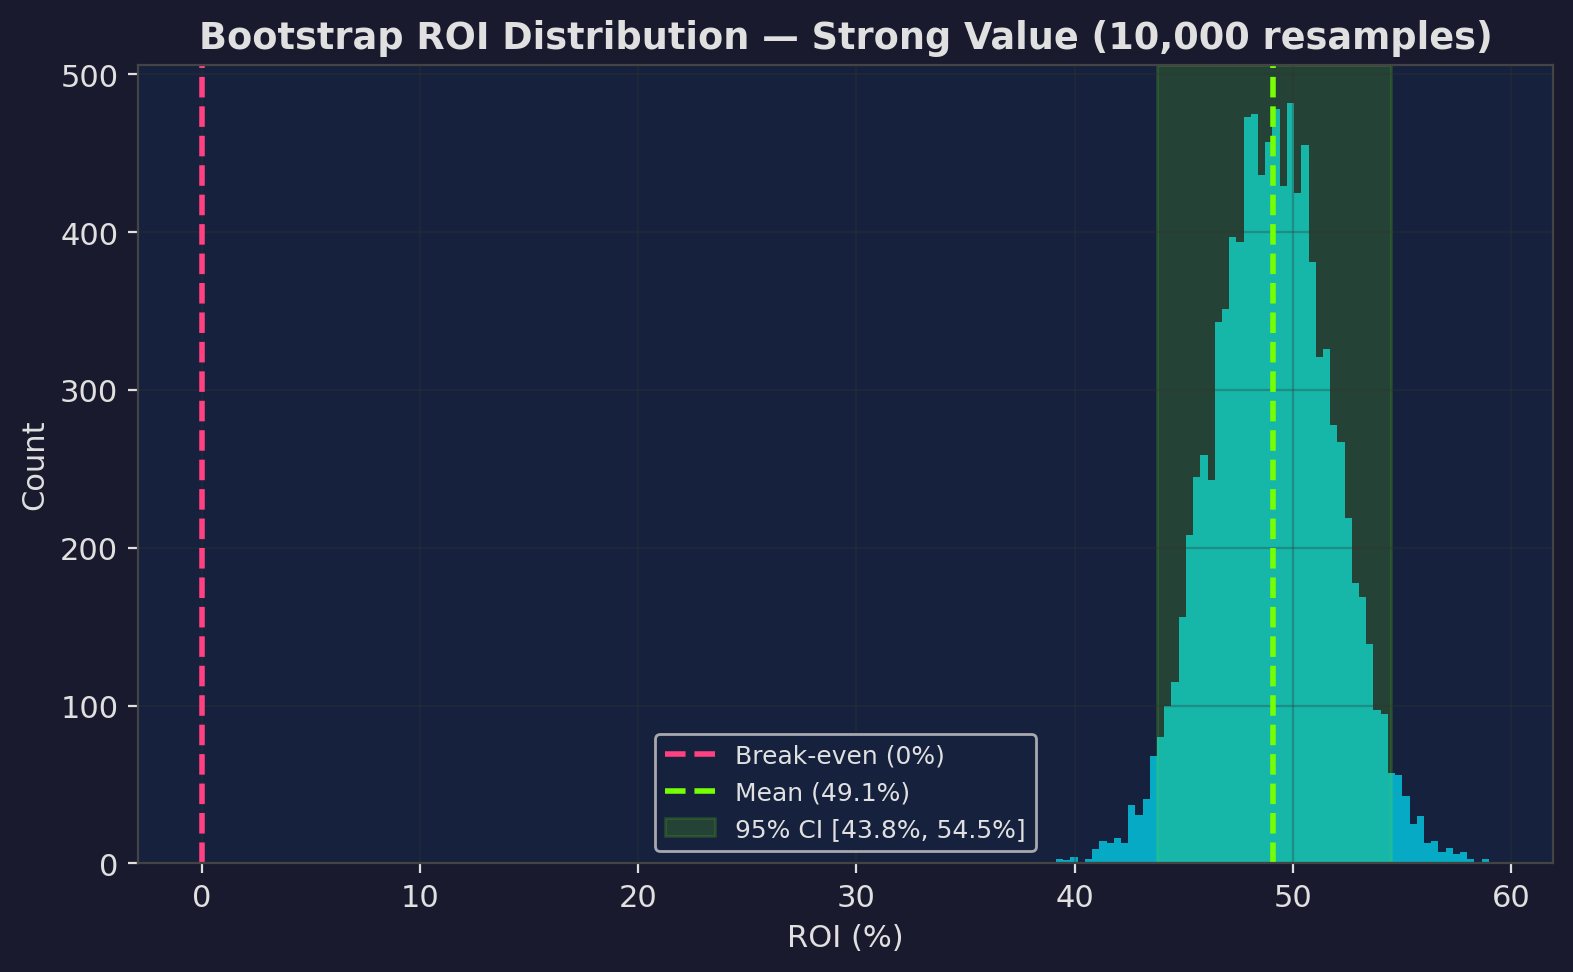
\includegraphics[width=0.75\textwidth]{figures/bootstrap.png}
\caption{Bootstrap ROI distribution (10,000 resamples). All resamples profitable.}
\end{figure}

\begin{table}[H]
\centering\small
\begin{tabular}{@{}lr@{}}
\toprule
\color{accent} Metric & \color{accent} Strong Value ($\geq$5\%) \\
\midrule
N bets & 3,340 \\
Observed ROI & +48.70\% \\
Bootstrap mean & +48.70\% \\
95\% confidence interval & [+43.37\%, +54.01\%] \\
P(profit $>$ 0) & 100.00\% \\
\bottomrule
\end{tabular}
\caption{Bootstrap statistics (10,000 resamples). ROI uses FT odds proxy --- see Section 10.}
\end{table}

% === SECTION 7: RECENT PERFORMANCE ===
\section{Recent Performance (Sep 2025 -- Feb 2026)}

\begin{figure}[H]
\centering
\begin{subfigure}[t]{0.48\textwidth}
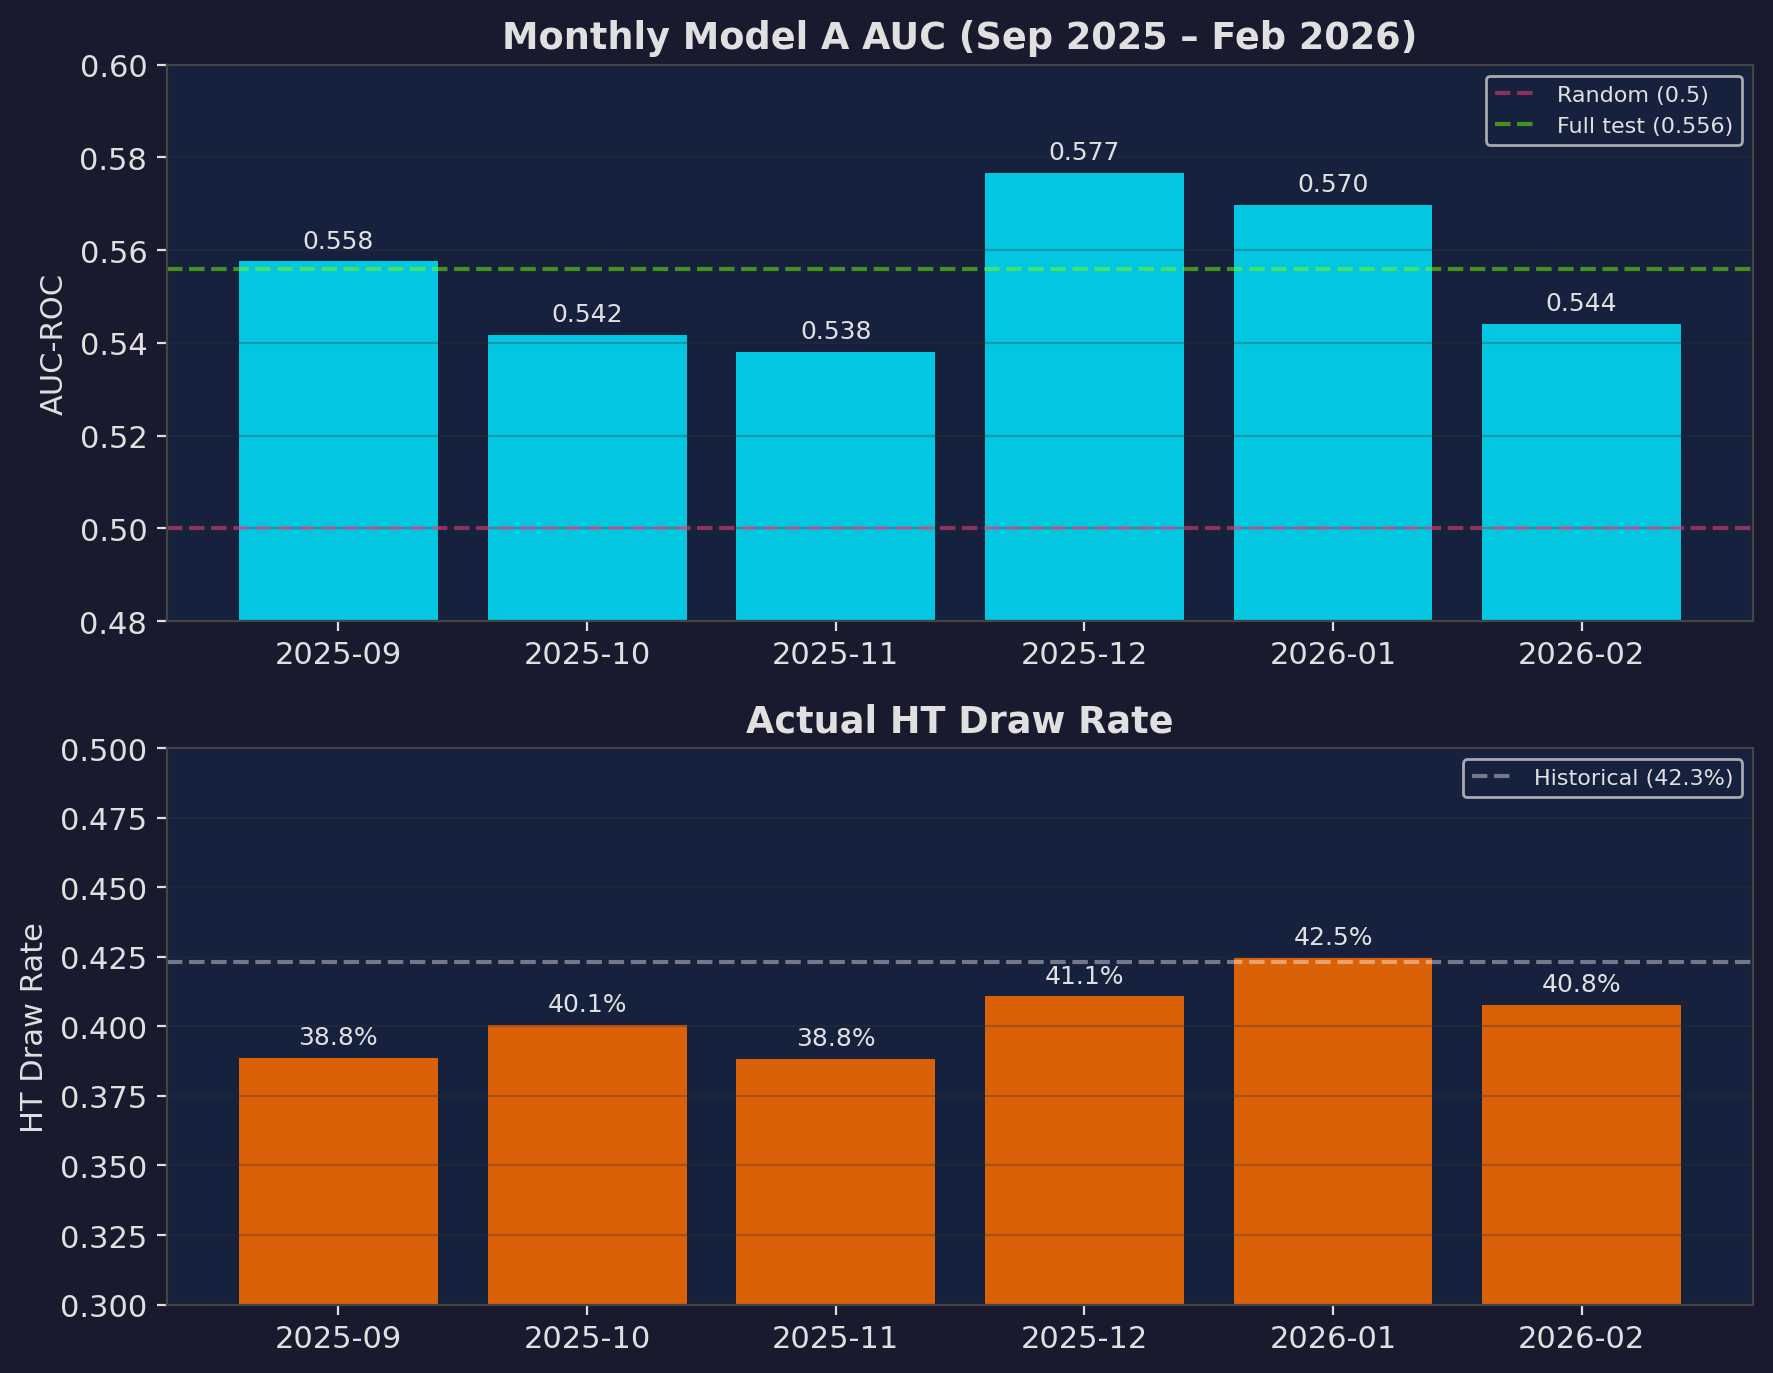
\includegraphics[width=\textwidth]{figures/monthly_recent.png}
\caption{Monthly AUC and draw rate.}
\end{subfigure}
\hfill
\begin{subfigure}[t]{0.48\textwidth}
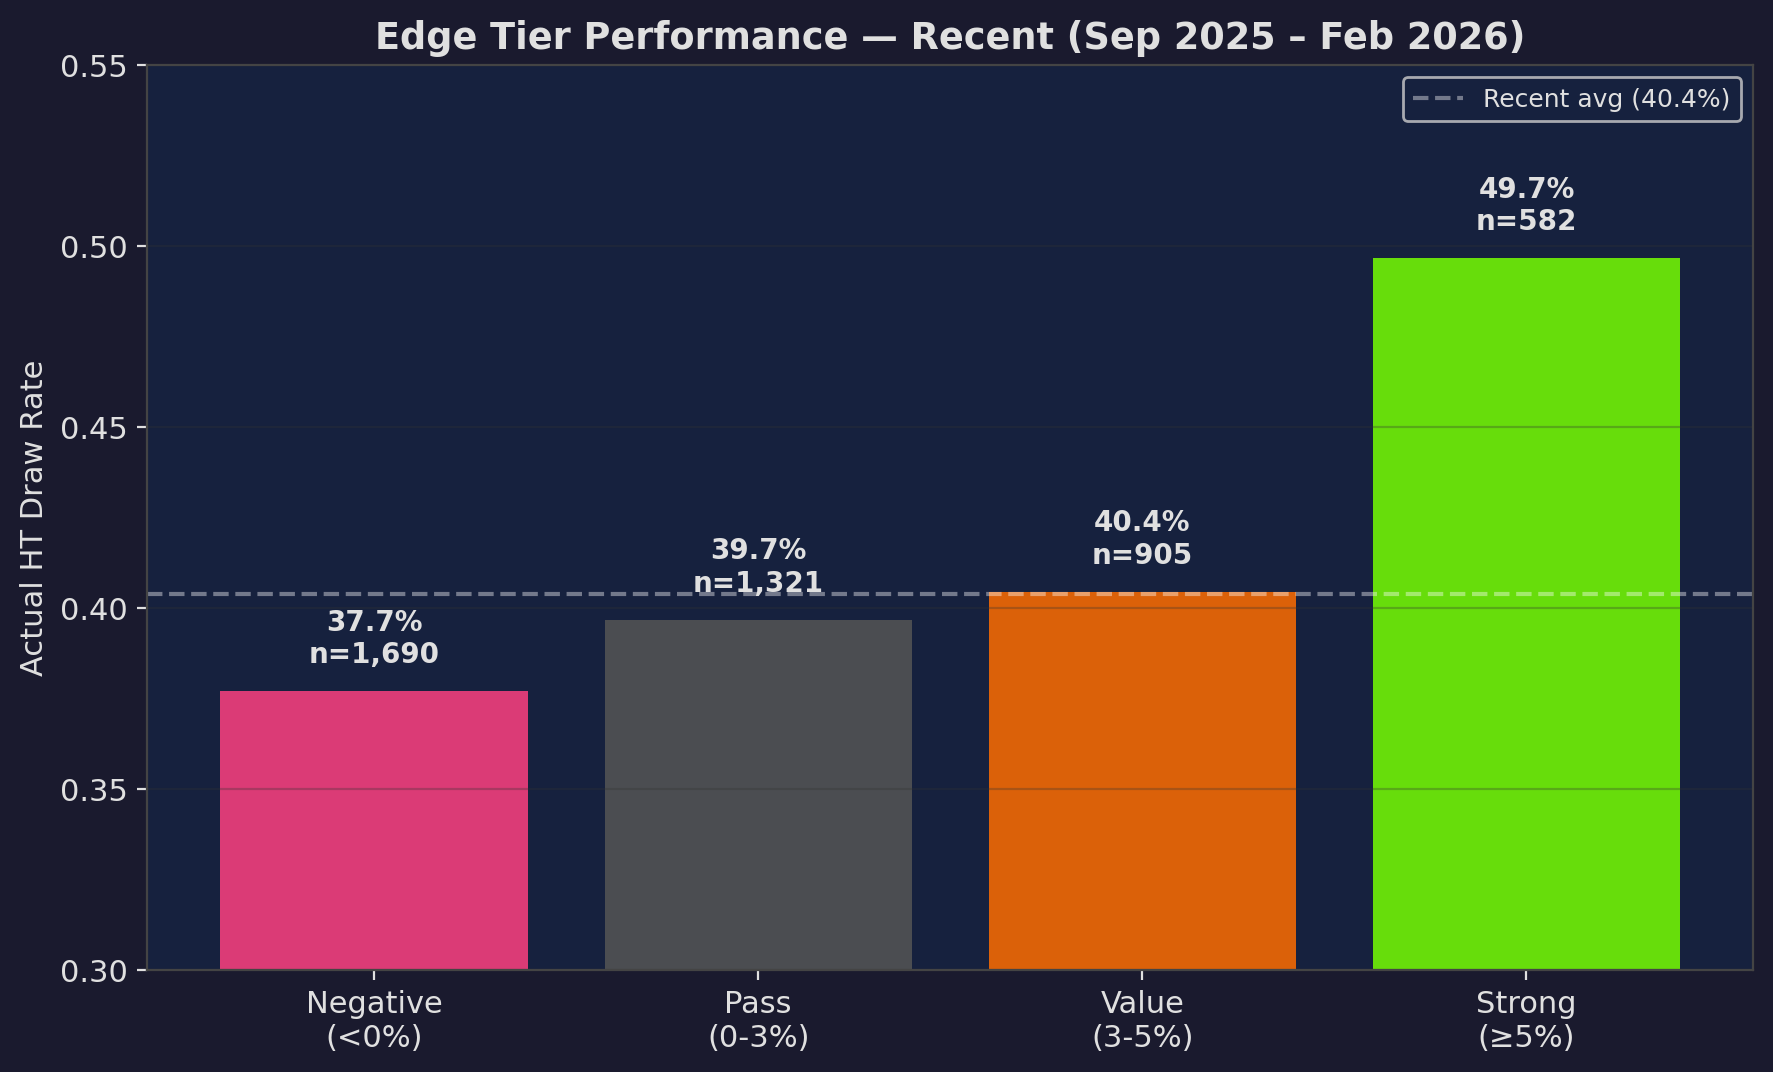
\includegraphics[width=\textwidth]{figures/edge_tiers_recent.png}
\caption{Edge tiers on recent data.}
\end{subfigure}
\end{figure}

\noindent On 4,498 recent matches, Strong Value ($\geq$5\% edge) achieves a \textbf{49.7\% hit rate} on 582 bets against a 40.4\% base rate --- a 9.3 percentage point lift. Monthly AUC ranges from 0.538 to 0.577, consistent with full test performance.

% === SECTION 8: CUMULATIVE PNL ===
\section{Cumulative Performance}

\begin{figure}[H]
\centering
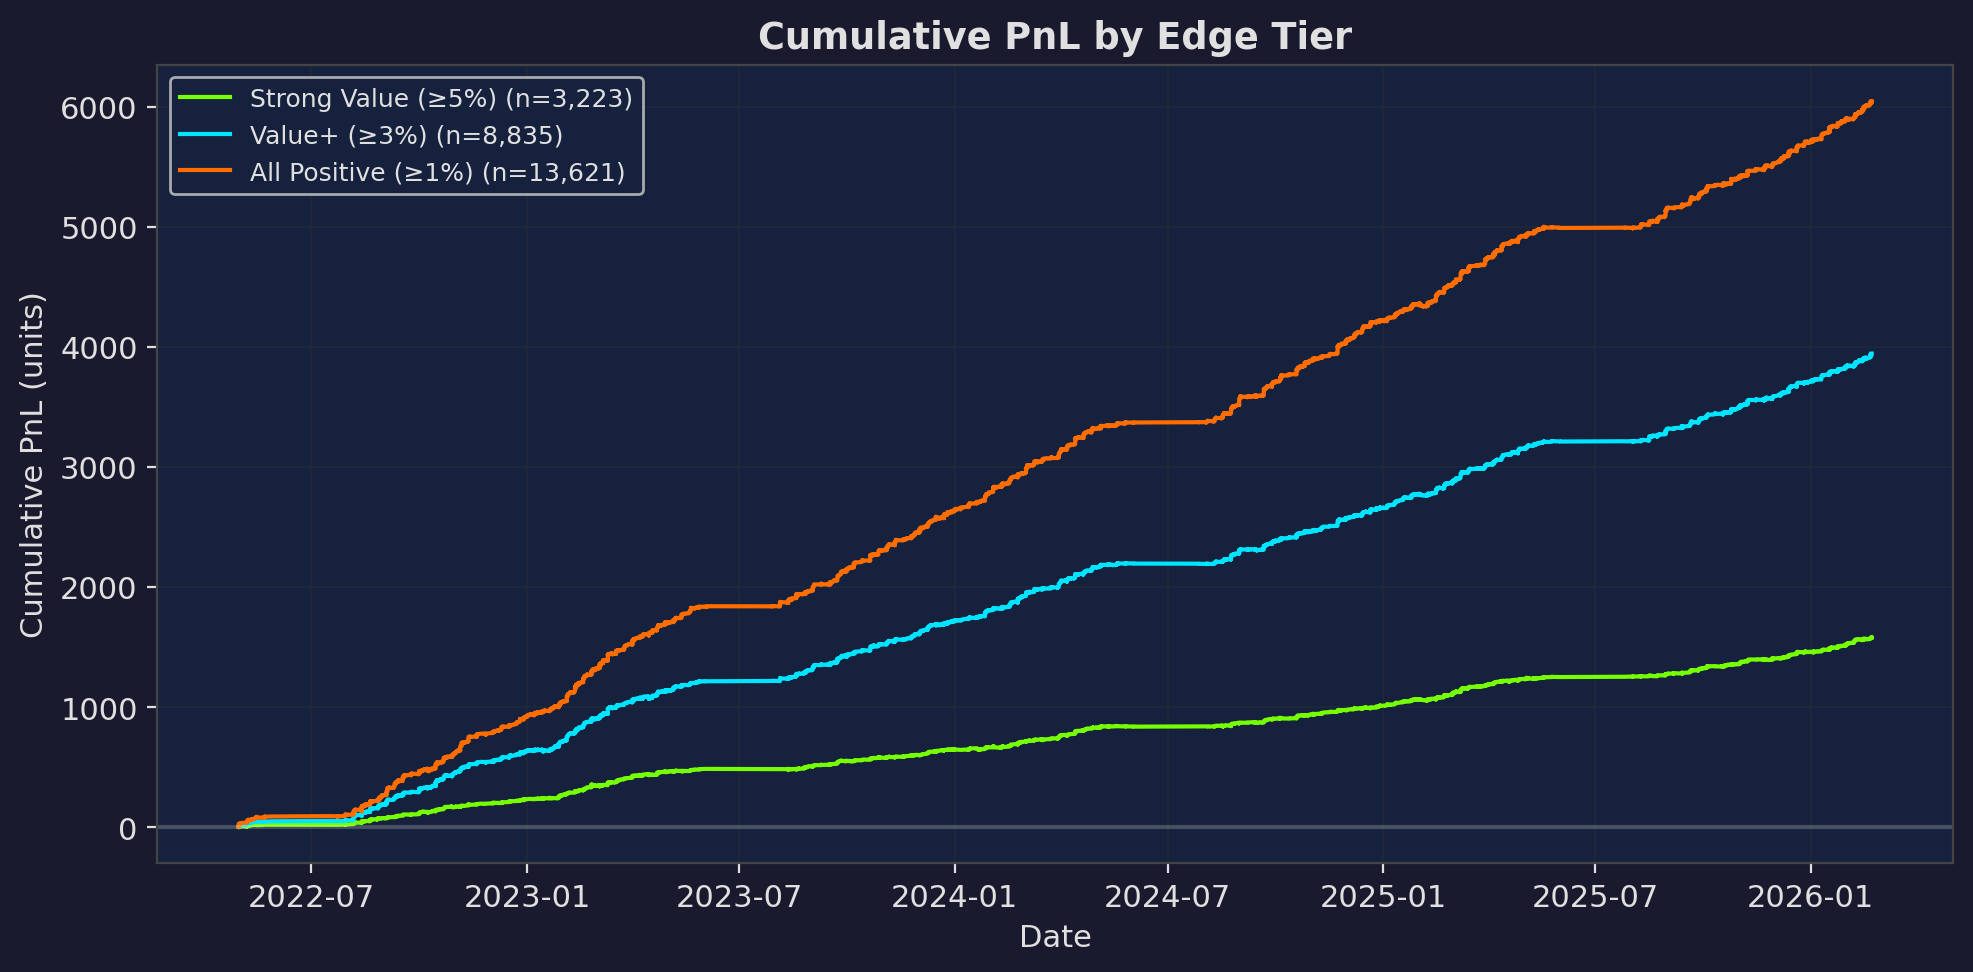
\includegraphics[width=0.85\textwidth]{figures/cumulative_pnl.png}
\caption{Cumulative PnL (units) by edge tier over the full test period.}
\end{figure}

% === SECTION 9: COMPUTATION ===
\section{Computation}

\begin{table}[H]
\centering\small
\begin{tabular}{@{}llr@{}}
\toprule
\color{accent} Operation & \color{accent} Hardware & \color{accent} Runtime \\
\midrule
Full training (Optuna 30 trials + 7 validations) & Apple M1 Pro, 16GB & 25s \\
Full backtest (30,025 matches, 16 quarterly DC/Elo refits) & " & 8m 21s \\
Prediction + analysis (29,120 matches) & " & 0.64s \\
Incremental data update & " & $<$5s \\
Single match prediction & " & $<$0.5s \\
\bottomrule
\end{tabular}
\caption{Compute benchmarks.}
\end{table}

\noindent Model artifacts total 8,067 KB. Dataset: 9.2 MB (Parquet). 22 European leagues from football-data.co.uk, 1995--2026.

% === SECTION 10: LIMITATIONS ===
\section{Limitations and Open Questions}

\begin{enumerate}[leftmargin=1.5em, itemsep=4pt]
  \item \textbf{FT odds proxy inflates all ROI figures.} This is the paper's most significant limitation. The backtest calculates payouts using B365 full-time draw odds (typically 3.0--3.5), but actual HT draw bets pay substantially less (typically 2.0--2.5 at US sportsbooks). This means reported ROI of +48.7\% is \textbf{not achievable in practice}. True ROI with real HT odds is unknown and could be negative after accounting for market vig.
  \item \textbf{Elo and Dixon-Coles default priors.} When team data is thin (e.g., promoted clubs, early season), both sub-models fall back to generic priors. The Elo model defaults to 42.0\% for many matches, reducing Model B to a single Dixon-Coles signal in those cases.
  \item \textbf{No transaction costs.} Bet availability, liquidity constraints, bookmaker limits, and odds movement between prediction time and bet placement are not modeled.
  \item \textbf{Prospective validation nascent.} 1 live bet placed, 3 days of tracking (Feb 2026). Real HT odds collection via The Odds API began Feb 2026. Minimum 3 months of prospective data needed to validate.
  \item \textbf{Potential look-ahead bias.} While train/val/test splits are strictly temporal, the choice of model architecture and hyperparameter ranges was informed by knowledge of the test period's existence. A truly blind test would require data that did not exist when modeling decisions were made.
\end{enumerate}

\subsection{What Is Validated}
The \textbf{hit rate staircase} is the paper's strongest claim. STRONG VALUE matches draw at HT 48.0\% of the time vs.\ a 40.7\% base rate, with monotonic improvement across all tiers. This ranking is computed purely from match outcomes and does not depend on odds. It is stable across all 9 half-year periods (range: 46.3\%--49.6\%).

\subsection{What Is Not Yet Validated}
Profitability. The edge may or may not survive real HT market odds and vig. Historical HT odds (2022--2026) are being collected from The Odds API to resolve this question. Updated results with real HT odds will be published as an addendum.

\vspace{8pt}
\noindent\colorbox{cardbg}{\parbox{\dimexpr\textwidth-2\fboxsep}{%
\color{accent}\textbf{Key open question:} Does the 48.0\% hit rate on STRONG VALUE produce positive ROI at real HT draw odds? At typical HT draw odds of +125 (2.25), a 48.0\% hit rate yields +8.0\% ROI before vig. At +100 (2.00), it yields -4.0\%. The answer depends on available HT market prices.}}

\vspace{16pt}
\noindent\rule{\textwidth}{0.4pt}
\begin{center}
\color{dimgray}\small
Source: \href{https://github.com/raulduk3/half-time}{github.com/raulduk3/half-time} · Data: football-data.co.uk · Model: V4 (Feb 2026)
\end{center}

\end{document}
